% !TEX root = ../main.tex
% NB: Bruker TikZ for grafen. Orkestrator: vennligst legg til
% \usepackage{tikz} i notes/preamble.tex hvis ikke allerede til stede.
\section{Q08: Tiltrekke og aflønne medarbeidere -- reservation utility, compensating differentials, superior assets, salary--fringe-mix}\label{q:08}

\begin{quote}
\emph{Redegør for hvordan virksomheder kan tiltrække og aflønne medarbejdere -- herunder også for begreberne reservation utility, compensating differentials, superior assets. Vis i forlængelse heraf en model til illustration af hvordan det optimale mix mellem salary og fringe benefits principielt kan håndteres.}
\end{quote}

\subsection*{Svar (kort)}
Bedriften tiltrekker og holder på ansatte ved å tilby en kompensasjonspakke som minst når kandidatens \thref{reservation-utility}{reservation utility} ($U_0$ -- nytten av neste-beste alternativ, dvs.\ ``gulvet'' for hva kandidaten aksepterer). Pakken justeres for \thref{compensating-differentials}{compensating differentials} (ekstra betaling for uattraktive jobbtrekk som nattskift, isolert lokasjon eller risiko), og bedriften utnytter \thref{superior-assets}{superior assets} (firmaspesifikke ressurser som lar den levere én krone nytte for mindre enn én krone kostnad -- f.eks.\ skala på helseforsikring, sterk merkevare, karrierevei). Pakken settes sammen av lønn $S$ og \emph{fringe benefits} $F$ (frynsegoder som pensjon, helse, ferie, bil, opsjoner). Optimal miks finnes der den ansattes indifferenskurve $U_0$ (kombinasjoner av $S$ og $F$ som gir lik nytte) \emph{tangerer} bedriftens isokostnadslinje (kombinasjoner som gir lik total kostnad for bedriften) -- altså der de to kurvene akkurat så vidt berører hverandre i ett punkt. I tangentpunktet kan ingen av partene få mer uten at den andre må gi opp noe. Dette er \thref{salary-fringe-benefits-mix}{salary--fringe-modellen}. [SLIDE]

\subsection*{Hvordan tiltrekke og aflønne (kort oversikt)}
\begin{itemize}\setlength{\itemsep}{2pt}
\item \textbf{Mål.} Kompensasjon skal (i) tiltrekke, (ii) retentere, (iii) motivere ansatte (BSZ kap.\ 14). [SLIDE]
\item \textbf{Gulvet.} Reservation utility $U_0$ = nytten av neste-beste alternativ. Pakken må over dette nivået, ellers takker kandidaten nei. [SLIDE]
\item \textbf{Pakkens dimensjoner.} Lønn $S$, fringe $F$ (pensjon, helse, ferie, bil, opsjoner), ikke-monetære goder (karrierevei, status, mening, kultur, jobbinnhold), arbeidsforhold. [SLIDE]
\item \textbf{Justeringer.} Uattraktive jobbtrekk $\Rightarrow$ compensating differential (mer $S$ eller målrettet $F$). Bedrifts-spesifikke styrker $\Rightarrow$ superior asset reduserer kostnad per nytte. [SLIDE]
\item \textbf{Mix-problemet.} Hvor stor andel $S$ vs.\ $F$? Avhenger av skatt, skala, ansattes preferanser. Optimum: tangering indifferens $\leftrightarrow$ isokost. [SLIDE]
\end{itemize}

\subsection*{Relevante teorier (kort)}

\paragraph{\thref{reservation-utility}{Reservation utility}\quad\SThree}
Minimumsnyttenivå $U_0$ kandidaten krever for å akseptere. Bestemmes av neste-beste alternativ pluss ikke-monetære faktorer (geografi, dual-career, status). Fungerer som \emph{participation constraint} i alle kontraktsproblemer: $U(\text{pakke}) \geq U_0$. Er kjernekoblingen mellom det ytre arbeidsmarkedet og bedriftens interne kompensasjonsdesign. Forklarer hvorfor bedrifter i pressmarkeder må overstige markedsnivå -- og hvorfor en sterk bedrift kan slippe med mindre kontantbeløp. [SLIDE]

\paragraph{\thref{compensating-differentials}{Compensating differentials}\quad\SThree}
Tillegg som må betales for jobber med uattraktive trekk: risiko, nattskift, isolert lokasjon, høyt stress, mye reising. Adam Smith (1776), formalisert i hedonisk lønnsteori (Rosen 1974). I likevekt fyller markedet uattraktive jobber bare fordi marginalkostnaden av disutility kompenseres. Forklarer offshore-tillegg, nattillegg, hardship allowance og hvorfor remote anlegg må tilby ekstra. [SLIDE/BOK]

\paragraph{\thref{superior-assets}{Superior assets (firm-specific assets)}\quad\SOne/\SThree}
Firmaspesifikke ressurser som lar bedriften levere én krone nytte til den ansatte for mindre enn én krone i kostnad: skattefavør på fringe, skalarabatt på forsikring, arbeidsgivermerkevare (\emph{employer brand}), kultur, internt arbeidsmarked, karrierevei, langsiktig eiermodell. Konsekvens: to bedrifter som konkurrerer om samme kandidat har ulik isokostnadslinje (kurven for kombinasjoner som gir lik total kostnad). Bedriften med superior asset når $U_0$ med en kurve nærmere origo $\Rightarrow$ varig kostnadsfordel. Tilsvarer en \emph{VRIN}-ressurs (Barney 1991: \emph{Valuable, Rare, Inimitable, Non-substitutable} -- verdifull, sjelden, umulig å kopiere, ingen erstatninger) anvendt på arbeidsmarkedet. [SLIDE/BOK]

\paragraph{\thref{salary-fringe-benefits-mix}{Salary vs.\ fringe benefits-modellen}\quad\SThree}
Bedriften minimerer kostnad $C(S,F) = c_S S + c_F F$ (én krone lønn koster $c_S$, én krone fringe koster $c_F$ -- ulike fordi skatt og skala kan gi rabatt på fringe) under bibetingelsen at den ansatte må få minst sin reservation utility: $U(S,F) \geq U_0$. Optimum: $\mathrm{MRS}_{S,F} = c_S/c_F$, der MRS er \emph{marginal substitusjonsrate} -- hvor mye fringe den ansatte er villig til å bytte mot én ekstra krone lønn på indifferenskurven. Sagt enkelt: i optimum er den ansattes byttekurs mellom $S$ og $F$ akkurat lik bedriftens kostnadskurs. Geometrisk: tangering mellom indifferenskurve og isokostnadslinje. Hvis $c_F < c_S$ (på grunn av skattefavør eller skalarabatt), tippes miksen mot mer $F$. Heterogene preferanser hos ulike ansatte begrunner \emph{cafeteria-style benefits} -- der den ansatte selv velger sammensetning. Modellen er den ``prinsipielle håndteringen'' spørsmålet ber om. [SLIDE/BOK]

\subsection*{Illustrasjoner fra forelesning}

\begin{figure}[H]
  \centering
  
\includegraphics[width=0.55\linewidth]{BSZ_kap_14_2026/by_slide/slide_002/BSZ_kap_14_2026_slide_002_asset_01_image1.jpeg}
  \caption{``I don't get out of bed for less than \$10,000 a day'' -- Linda Evangelista. Illustrerer reservation utility: minimumsnytten en kandidat krever for å akseptere. (BSZ kap.\ 14, slide 2) [SLIDE]}
\end{figure}

\begin{figure}[H]
  \centering
  
\includegraphics[width=0.5\linewidth]{BSZ_kap_14_2026/by_slide/slide_014/BSZ_kap_14_2026_slide_014_asset_01_image5.jpeg}
  \caption{Mengenrabatt -- illustrerer superior assets: bedrifter med skalafordeler kan levere fringe benefits billigere per nyttekrone enn konkurrenten. (BSZ kap.\ 14, slide 14) [SLIDE]}
\end{figure}

\subsection*{Grafisk modell -- optimal lønnsmix}

\begin{figure}[H]
  \centering
  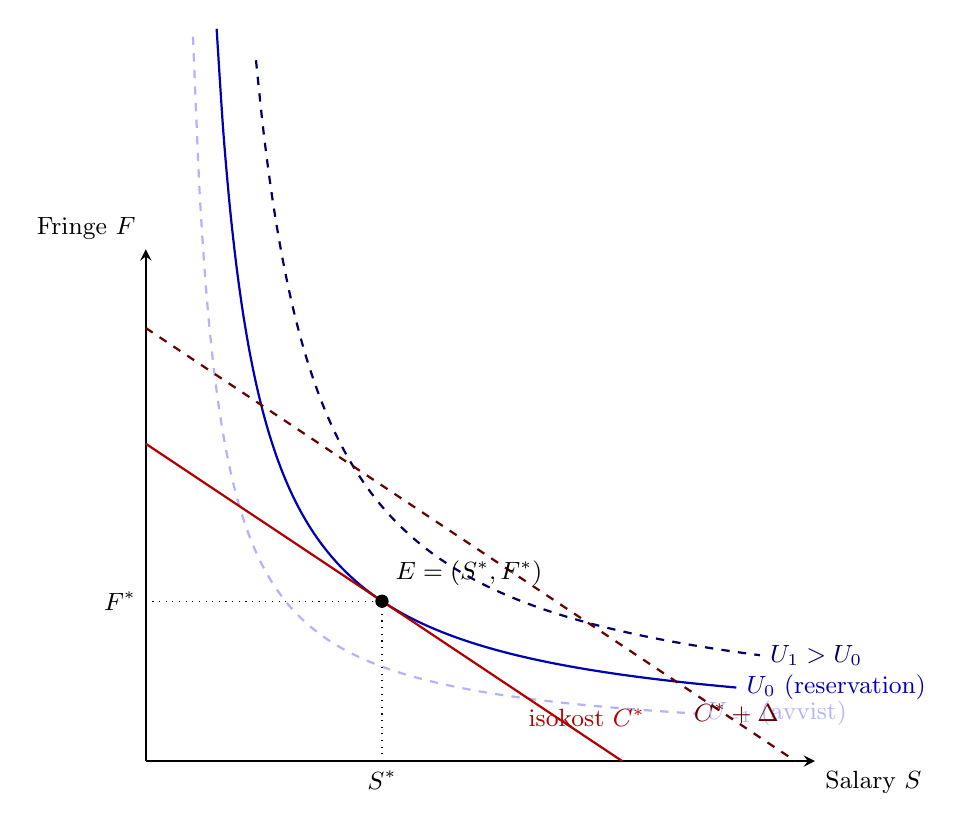
\begin{tikzpicture}[scale=1.0, >=stealth]
    \draw[->, thick] (0,0) -- (8.5,0) node[below right] {\small Salary $S$};
    \draw[->, thick] (0,0) -- (0,6.5) node[above left] {\small Fringe $F$};

    % Indifferenskurver
    \draw[blue!70!black, thick, domain=0.9:7.5, smooth, samples=80]
      plot (\x, {4.5/(\x-0.4) + 0.3}) node[right] {\small $U_0$ (reservation)};
    \draw[blue!40!black, thick, dashed, domain=1.4:7.8, smooth, samples=80]
      plot (\x, {6.8/(\x-0.6) + 0.4}) node[right] {\small $U_1 > U_0$};
    \draw[blue!30, thick, dashed, domain=0.6:7.0, smooth, samples=80]
      plot (\x, {2.7/(\x-0.3) + 0.2}) node[right] {\small $U_{-1}$ (avvist)};

    % Isokost
    \draw[red!70!black, thick] (0, 4.03) -- (6.05, 0);
    \node[red!70!black] at (5.6, 0.55) {\small isokost $C^*$};
    \draw[red!40!black, thick, dashed] (0, 5.5) -- (8.25, 0);
    \node[red!40!black] at (7.5, 0.6) {\small $C^* + \Delta$};

    % Optimum
    \filldraw[black] (3, 2.03) circle (2.2pt);
    \node[anchor=south west] at (3.05, 2.1) {\small $E = (S^*, F^*)$};
    \draw[dotted] (3, 0) -- (3, 2.03);
    \draw[dotted] (0, 2.03) -- (3, 2.03);
    \node[below] at (3, 0) {\small $S^*$};
    \node[left] at (0, 2.03) {\small $F^*$};
  \end{tikzpicture}
  \caption{Optimal mix mellom lønn $S$ og fringe $F$. Konvekse indifferenskurver $U_{-1}, U_0, U_1$ reflekterer at $S$ og $F$ er imperfekte substitutter i ansattes nytte. Isokostnadslinjer har helning $-c_S/c_F$. Optimum $E$: laveste isokost som berører $U_0$. Hvis $c_F$ synker (skatt, skala, superior asset) blir isokost flatere $\Rightarrow$ mer $F^*$, mindre $S^*$. Hvis $U_0$ stiger (stramt marked) flyttes hele kurven utover $\Rightarrow$ høyere total kostnad. [SLIDE]}
\end{figure}

\textbf{Tolkning:} I tangeringspunktet $E$ er ansattes marginale substitusjonsrate mellom lønn og fringe akkurat lik bedriftens kostnadsforhold mellom dem. Bedriften kan ikke spare penger ved å vri mixen uten å falle under $U_0$. Heterogene preferanser gir ulike indifferenskurver $\Rightarrow$ ulik optimal mix per ansatt $\Rightarrow$ rasjonale for cafeteria-style benefits. [SLIDE]

\subsection*{Real-world eksempler}

\textbf{Eks.~1 -- Equinor vs.\ Goldman Sachs (skandinavisk vs.\ angloamerikansk lønnsmix).}\quad [EKS]
For tilsvarende analytiker-/ingeniørprofiler tilbyr Equinor moderat kontantlønn, men tung fringe: omfattende pensjon via Statens pensjonskasse-aktig struktur, helseforsikring, lang ferie, langsiktig karrierevei på tvers av olje/gass/fornybar. Goldman Sachs tilbyr motsatt mix: høy grunnlønn + stor variabel bonus, lite formell fringe, kortere ansiennitetsfordeler. Forskjellen reflekterer (i) ulik $c_F$ (skandinavisk skattefavør og skala på Equinor; mindre fordel i USA), (ii) ulik $U_0$ for målgruppene (Goldman-kandidatens alternativ er hedge funds; Equinor-kandidatens er andre nordiske energiselskaper), og (iii) ulike superior assets -- Equinor har langsiktig stabilitet, Goldman har prestisje og prestasjons-signaling. Begge er optimum gitt egne $c_S, c_F, U_0$ og preferanser; ingen er ``riktig''.

\textbf{Eks.~2 -- Novo Nordisk vs.\ ung biotech-startup.}\quad [EKS]
Novo Nordisk har et superior asset i form av forskningsmiljø (eneste i verdensklasse innen diabetes), skala på fringe (helse, barnepass, kantine), og stiftelsesstabilitet -- en biokjemiker får høy ikke-monetær nytte og rimelige fringe-goder. Optimum: moderat $S^*$, høyt $F^*$, og lav total kostnad relativt til $U_0$. Ung biotech-startup (f.eks.\ Evaxion eller mindre Medicon Valley-aktør) mangler disse assetene -- må kompensere med høyere kontant grunnlønn og opsjoner, fordi $c_F$ er høy (ingen skala) og ikke-monetær superior asset er svakere. Samme markedskandidat, samme $U_0$, men ulike isokostnadslinjer $\Rightarrow$ ulike optimale mix.

\subsection*{Kobling til Mærsk Power-to-X}\quad [CASE]
PtX-divisjonen konkurrerer om scarce elektrolyse- og prosjektingeniør-talent mot Ørsted, Siemens Energy, Topsoe og Hydrogen-startups. \textbf{Reservation utility} settes i hjemmemarkedet av Ørsted (renomme i havvind, danske forhold). Mærsk PtX må overstige $U_0$, men ikke nødvendigvis ved å matche Ørsteds lønn krone for krone -- de vrir mixen mot fringe og ikke-monetære goder der Mærsks \textbf{superior assets} er rimeligere å levere enn for konkurrenten: (i) global merkevare og krysskonsern-karrierevei (shipping $\to$ logistikk $\to$ PtX $\to$ Maersk Energy), (ii) stiftelseseier som signaliserer langsiktig jobbsikkerhet, (iii) København-HQ-velferdsgoder (kantine, sentral lokasjon, familiefringe), (iv) prestisje fra A.P.\ Møller-tradisjonen. \textbf{Compensating differentials} er i tillegg relevant fordi mange PtX-anlegg vil ligge avsidesliggende (havvindkobling, areal, billig strøm) -- her må Mærsk legge på lokasjons-tillegg eller fly-in/fly-out-ordninger. Resultatet er et $(S^*, F^*)$-optimum med mer $F$ og mindre $S$ enn Ørsteds, til lavere total kostnad per ansatt -- forutsatt at superior assetene faktisk leverer reell nytte.

\subsection*{Fallgruber}
\begin{itemize}\setlength{\itemsep}{2pt}
\item Glemme at $U_0$ er en \emph{indifferenskurve}, ikke et lønnsbeløp -- multidimensjonal.
\item Forveksle compensating differentials med ren risikopremie i \thref{principal-agent}{prinsipal--agent}; det første kompenserer for jobbtrekk, det andre for risikoeksponering.
\item Påstå at fringe alltid er optimalt -- forutsetter $c_F < c_S$ (skatt, skala) og passende preferanser.
\item Tegne indifferenskurver konkave eller rette i stedet for konvekse.
\item Glemme at superior asset \emph{må} levere reell nytte for at det skal funke -- ellers er ``kultur'' bare et påskudd for å betale mindre.
\item Glemme at heterogene preferanser begrunner cafeteria-style design.
\item Behandle modellen som statisk -- $U_0$, $c_S$ og $c_F$ endrer seg med konjunktur, skatt og bedriftens livssyklus.
\item Hoppe over grafen -- spørsmålet ber eksplisitt om å \emph{vise en modell}.
\end{itemize}

\FloatBarrier
\subsection*{Håndskrivbar disposisjon (15-min forberedelse)}

\begin{figure}[H]
  \centering
  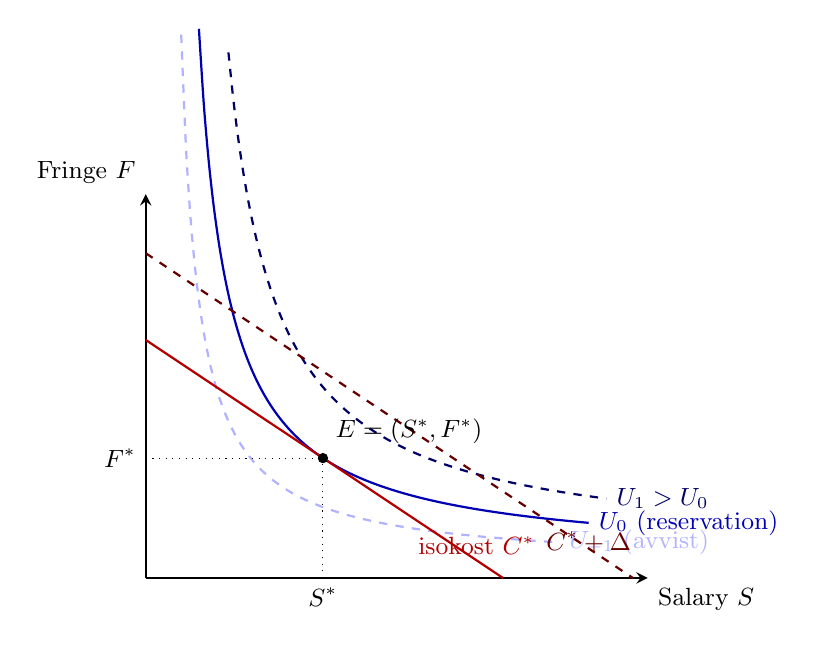
\begin{tikzpicture}[scale=0.75, >=stealth]
    \draw[->, thick] (0,0) -- (8.5,0) node[below right] {\small Salary $S$};
    \draw[->, thick] (0,0) -- (0,6.5) node[above left] {\small Fringe $F$};

    % Indifferenskurver
    \draw[blue!70!black, thick, domain=0.9:7.5, smooth, samples=80]
      plot (\x, {4.5/(\x-0.4) + 0.3}) node[right] {\small $U_0$ (reservation)};
    \draw[blue!40!black, thick, dashed, domain=1.4:7.8, smooth, samples=80]
      plot (\x, {6.8/(\x-0.6) + 0.4}) node[right] {\small $U_1 > U_0$};
    \draw[blue!30, thick, dashed, domain=0.6:7.0, smooth, samples=80]
      plot (\x, {2.7/(\x-0.3) + 0.2}) node[right] {\small $U_{-1}$ (avvist)};

    % Isokost
    \draw[red!70!black, thick] (0, 4.03) -- (6.05, 0);
    \node[red!70!black] at (5.6, 0.55) {\small isokost $C^*$};
    \draw[red!40!black, thick, dashed] (0, 5.5) -- (8.25, 0);
    \node[red!40!black] at (7.5, 0.6) {\small $C^* + \Delta$};

    % Optimum
    \filldraw[black] (3, 2.03) circle (2.2pt);
    \node[anchor=south west] at (3.05, 2.1) {\small $E = (S^*, F^*)$};
    \draw[dotted] (3, 0) -- (3, 2.03);
    \draw[dotted] (0, 2.03) -- (3, 2.03);
    \node[below] at (3, 0) {\small $S^*$};
    \node[left] at (0, 2.03) {\small $F^*$};
  \end{tikzpicture}
  \caption{Salary--fringe-modellen (referansefigur for disposisjonen): konvekse indifferenskurver, rett isokost, optimum $E$ i tangeringspunktet. [SLIDE]}
\end{figure}

\begin{itemize}\setlength{\itemsep}{2pt}
\item \textbf{Tese:} Kompensasjon = sett sammen pakke ($S, F$, ikke-monetær) som passerer $U_0$ til lavest kostnad. Optimum = tangering indifferenskurve $\leftrightarrow$ isokost.
\item \textbf{Mål med kompensasjon:} tiltrekke, retentere, motivere.
\item \textbf{\thref{reservation-utility}{Reservation utility} $U_0$:} gulv, neste-beste alternativ, multidimensjonal, participation constraint.
\item \textbf{\thref{compensating-differentials}{Compensating differentials}:} tillegg for uattraktive trekk (risiko, skift, isolasjon). Adam Smith $\to$ Rosen 1974.
\item \textbf{\thref{superior-assets}{Superior assets}:} firmaspesifikke fordeler som senker $c_F$ -- skatt, skala, brand, kultur, karrierevei.
\item \textbf{\thref{salary-fringe-benefits-mix}{Salary--fringe-modellen}:} $\min c_S S + c_F F$ s.t. $U(S,F) \geq U_0 \Rightarrow \mathrm{MRS} = c_S/c_F$.
\item \textbf{Graf:} indifferens $U_0$ konveks, isokost rett, optimum $E$ tangering, dotted projeksjoner til $S^*, F^*$.
\item \textbf{Heterogene preferanser:} ulike kurver $\Rightarrow$ cafeteria-style benefits.
\item \textbf{Eks.\ 1:} Equinor (mye fringe) vs.\ Goldman (mye $S$). Ulike $c_F$, $U_0$, superior assets.
\item \textbf{Eks.\ 2:} Novo Nordisk (forskningsmiljø + skala) vs.\ liten biotech (må overby på $S$).
\item \textbf{Case Mærsk PtX:} $U_0$ satt av Ørsted; superior assets (brand, krysskonsern, stiftelse, HQ) lar dem vri mot $F$; compensating differential for remote anlegg.
\item \textbf{Søyle:} \SThree\ primært; \SOne\ via karriere-/rolleallokering.
\end{itemize}
